\section{Properties of the perceptron}

\subsection{Model structure}

A perceptron is a layered feed-forward neural network. A connection originating from any given unit in the network can only lead to a unit in the next layer, as shown in Fig. 1.

A $K$-layer network contains a layer of input units, a layer of output units and $K-1$ layers of hidden units between them. A simple perceptron is a single-layer network with no hidden layers, as shown in Fig. 1(b). A simple perceptron with $N$-dimensional input $\xi = (\xi_1, \xi_2, ... \xi_N)$ and $M$-dimensional output $O = (O_1, ..., O_M)$ computes the output in the following way:

\begin{equation}
    O_i = g(h_i) = g \left( \sum_{j=1}^N \xi_j w_{ij} \right)
\end{equation}

The $w_{ij}$ factors are the components of the weight vector $w_i$ and $g(\cdot)$ is the activation function. $g(\cdot)$ is usually a non-linear threshold function. We will henceforth use $g(h) = \mathrm{sgn} (h)$ as our activation function.

We will not take into account any biases for simple perceptrons, as having bias element is equivalent to having an $(N+1)$-dimensional input and setting $\xi_{N+1} = -1$.

Perceptrons are used for supervised learning, that is, given a training set of $p$ input-output patterns, with input $\xi$ and output $\zeta$, we want the following to be true for every $i = 1, 2, ..., M$ and $\mu = 1, 2, ..., p$:

\begin{equation}
    O_i^\mu = \zeta_i^\mu
\end{equation}

We assume that target outputs $\zeta_i^\mu \in \{ \pm 1 \}$. Thus the problem in (2) is reduced to requiring that the signs of $h_i^\mu$ and $\zeta_i^\mu$ be the same for every $i$ and $\mu$. We suppose that output units are i.i.d., so we can drop the $i$ subscripts without loss of generality. Thus, for every $\mu$, we can reformulate (2) as:

\begin{equation}
    sgn(w \cdot \xi^\mu) = \zeta^\mu
\end{equation}

This implies that every input $\xi^\mu$ projected onto $w$ has the same sign as $\zeta^\mu$. Positive and negative projections onto $w$ are separated by the hyperplane that is perpendicular to $w$ and goes through the origin. For a perceptron to learn all the input-output patterns in the training set, this hyperplane must divide the inputs that have positive and negative targets, as shown in Fig. 2.

\begin{center}
\begin{figure}[bhtp]
    \centering
    \captionsetup{justification=centering, font=small, margin=0.5cm}
    \begin{subfigure}[b]{0.52\linewidth}
        \centering
        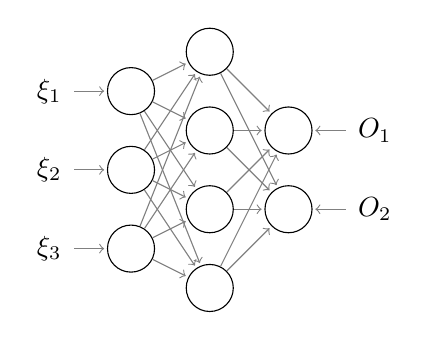
\begin{tikzpicture}[scale=1, shorten >=1pt,->,draw=black!50, node distance=1cm]
    \tikzstyle{every pin edge}=[<-,shorten <=1pt]
    \tikzstyle{neuron}=[circle,fill=black!25,minimum size=17pt,inner sep=0pt]
    \tikzstyle{input neuron}=[neuron, draw=black, fill=white!50];
    \tikzstyle{output neuron}=[neuron, draw=black, fill=white!50];
    \tikzstyle{hidden neuron}=[neuron, draw=black, fill=white!50];
    
    % Draw the input layer nodes
    \foreach \name / \y in {1,...,3}
    % This is the same as writing \foreach \name / \y in {1/1,2/2,3/3,4/4}
        \node[input neuron, pin=left:$\xi_{\y}$] (I-\name) at (0,-\y) {};

    % Draw the hidden layer nodes
    \foreach \name / \y in {1,...,4}
        \path[yshift=0.5cm]
            node[hidden neuron] (H-\name) at (1cm,-\y cm) {};
            
    % Draw the output layer node
    \node[output neuron, pin=right:$O_1$, right of=H-2] (O-1) {};
    \node[output neuron, pin=right:$O_2$, right of=H-3] (O-2) {};

    % Connect every node in the input layer with every node in the hidden layer.
    \foreach \source in {1,...,3}
        \foreach \dest in {1,...,4}
            \path (I-\source) edge (H-\dest);

    % Connect every node in the hidden layer with the output layer
    \foreach \source in {1,...,4}
        \foreach \dest in {1,...,2}
        \path (H-\source) edge (O-\dest);

\end{tikzpicture}
        \caption{Two-layer perceptron}
    \end{subfigure}
    \begin{subfigure}[b]{0.46\linewidth}
        \centering
        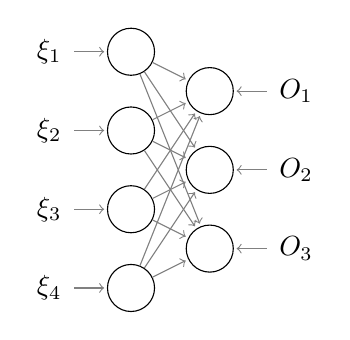
\begin{tikzpicture}[scale=1, shorten >=1pt,->,draw=black!50, node distance=1cm]
    \tikzstyle{every pin edge}=[<-,shorten <=1pt]
    \tikzstyle{neuron}=[circle,fill=black!25,minimum size=17pt,inner sep=0pt]
    \tikzstyle{input neuron}=[neuron, draw=black, fill=white!50];
    \tikzstyle{output neuron}=[neuron, draw=black, fill=white!50];
    
    % Draw the input layer nodes
    \foreach \name / \y in {1,...,4}
    % This is the same as writing \foreach \name / \y in {1/1,2/2,3/3,4/4}
        \node[input neuron, pin=left:$\xi_{\y}$] (I-\name) at (0,-\y) {};

    % Draw the hidden layer nodes
    \foreach \name / \y in {1,...,3}
        \path[yshift=-0.5cm]
            node[output neuron, pin=right:$O_\y$] (O-\name) at (1cm,-\y cm) {};
    
    % Connect every node in the input layer with every node in the hidden layer.
    \foreach \source in {1,...,4}
        \foreach \dest in {1,...,3}
            \path (I-\source) edge (O-\dest);
\end{tikzpicture}
        \caption{Simple perceptron}
    \end{subfigure}
    \caption{Examples of perceptrons}
    \label{fig:1}
\end{figure}
\end{center}

We can clearly see that the solvability of a problem by a simple perceptron depends on whether the problem is linearly separable or not. A linearly separable problem is one where there exists a hyperplane dividing the input-output patterns with output units $\zeta^\mu = -1$ from those with output units $\zeta^\mu = 1$. Since we are not working with biases, the separating hyperplane must pass through the origin. In the case of multiple units, such a hyperplane must exist for each output unit.

\begin{center}
\begin{figure}[thbp]
\centering
\captionsetup{justification=centering, font=small, margin=0.5cm}
\begin{tikzpicture}
\begin{axis}[
    axis lines=middle,
    xmin=-10, xmax=10,
    ymin=-8, ymax=8,
    xlabel=$\xi_1$, ylabel=$\xi_2$,
    xtick=\empty, ytick=\empty
]
\addplot [only marks] table {
-8 -4
-6  2
-4  5   
-3  7
-2  3
2  6
};
\addplot [only marks, mark=o] table {
-3  -5
3  -7
1  -4
5   -3
6   3
7   -1
};
\addplot [domain=-6:6, samples=2, dashed] {x};
\addplot [domain=0:2, samples=2, -stealth] {-x} node[above right] {$w$};
\end{axis}
\end{tikzpicture}
\caption{For $N=2$, output targets $\zeta^\mu$ are divided by a hyperplane perpendicular to $w$, passing through the origin. Adapted from \cite[p.93]{introbook}}
\label{fig:2}
\end{figure}
\end{center}

\subsection{Learning algorithm}

The perceptron learning algorithm is the procedure through which the perceptron finds an appropriate weight vector $w$ to satisfy (3).\footnote[1]{We assume a single output unit, but the algorithm can be easily generalized for multiple output units}

We begin with a null vector $w$. Then, iterating over the inputs $\xi_j^\mu$, we verify whether the output units correspond to the desired ones. If the output unit $O^\mu$ corresponds to the desired output unit $\zeta^\mu$, we do not change the value of the weight vector element feeding into that output unit. Otherwise, we update the weight vector as follows:

\begin{equation}
    w_{j}^{new} = w_{j}^{old} + \Delta w_{j}
\end{equation}

\noindent where:

\begin{equation}
    \Delta w_{j} = \eta (\zeta^{\mu} - O^{\mu}) \xi_j^{\mu}
\end{equation}

\noindent with $\eta \ll 1$ defined as the learning rate of the perceptron.

Taking into consideration the possibility of small errors in the input patterns, we set a requirement that the output is greater than some predefined margin $\kappa > 0$. Combining this requirement with the condition that $h^\mu$ and $\zeta^\mu$ be of the same sign, we obtain the following condition to verify when updating the weight vector:

\begin{equation}
    \zeta^\mu h^\mu \equiv \zeta^\mu \sum_j w_{j} \xi_j^\mu > N \kappa
\end{equation}

Since the left-hand side of the inequality scales with $N$, we add $N$ to the right-hand side of the inequality, allowing $\kappa$ to be constant. The derivation of $\Delta w_{j}$ thus becomes:

\begin{equation}
    \Delta w_{j} = \eta \Theta(N \kappa - \zeta^\mu h^\mu) \zeta\mu \xi_j^{\mu}
\end{equation}

\noindent where $\Theta$ denotes the step function.

Equation (7) represents the perceptron learning rule, describing the way in which a perceptron updates the weight vector as it learns new patterns.